% Source - https://tex.stackexchange.com/a/140550
% Posted by Steven B. Segletes, modified by community. See post 'Timeline' for change history
% Retrieved 2026-06-05, License - CC BY-SA 4.0

\documentclass[lettersize,journal]{IEEEtran}
\usepackage{amsmath,amsfonts}
\usepackage{algorithmic}
\usepackage{algorithm}
\usepackage{array}
\usepackage[caption=false,font=normalsize,labelfont=sf,textfont=sf]{subfig}
\usepackage{textcomp}
\usepackage{stfloats}
\usepackage{url}
\usepackage{verbatim}
\usepackage{graphicx}
\usepackage{cite}
\usepackage[colorlinks=true,linkcolor=blue,citecolor=blue,urlcolor=blue]{hyperref}
\usepackage{xcolor}

\usepackage{stackengine,scalerel}
\newlength\shlength
\newcommand\MyRVec[2][0]{\ThisStyle{\setlength\shlength{#1\LMpt}%
  \stackengine{-1.3ex}{$\SavedStyle#2$}{\smash{$\kern\shlength%
    \stackengine{1.55ex}{$\SavedStyle\raisebox{0.24ex}{$\mathchar"017E$}$}%
      {\rule{\widthof{$\SavedStyle#2$}}{\dimexpr.02ex+.1ex}\kern+0.20ex}{O}{r}{F}{F}{L}\kern-\shlength$}}%
      {O}{c}{F}{T}{S}}}
\newcommand\MyLVec[2][0]{\ThisStyle{\setlength\shlength{#1\LMpt}%
  \stackengine{-1.3ex}{$\SavedStyle#2$}{\smash{$\kern\shlength%
    \stackengine{1.55ex}{\kern-0.46ex\raisebox{0.24ex}{\reflectbox{\ensuremath{\mathchar"017E}}}}%
      {\kern-0.25ex\rule{\widthof{$\SavedStyle#2$}}{\dimexpr.02ex+.1ex}}{O}{l}{F}{F}{L}\kern-\shlength$}}%
      {O}{c}{F}{T}{S}}}

\usepackage[normalem]{ulem}
\newcommand{\hluline}[1]{\stackunder[-0.4pt]{#1}{\rule{\widthof{#1}}{0.4pt}}}

\hyphenation{op-tical net-works semi-conduc-tor IEEE-Xplore}

\begin{document}
\[ \vec{A} \quad \MyRVec[1]{ABC} \quad \MyRVec[1]{H} \quad \MyRVec[1]{H^{(l)}_{i}} \quad \MyRVec[1]{xyz} \quad \MyRVec{\Omega M} \]

% Mũi tên phải → trái
\[ \MyLVec[1]{A} \quad \MyLVec[1]{ABC} \quad \MyLVec[1]{H} \quad \MyLVec[1]{H^{(l)}_{i}} \quad \MyLVec[1]{xyz} \quad \MyLVec{\Omega M} \]


As illustrated in Fig., BiDecT represents each input video as a sequence of GOPs rather than densely sampled individual frames, reducing temporal redundancy while preserving local spatio-temporal structure. The overall framework consists of four main components. First, the Multimodal Feature Extraction module derives three complementary modalities—appearance, semantic, and motion—from all GOPs in the video. Second, the Multimodal Feature Embedding module projects these modalities into a shared representation space and combines them into a unified multimodal representation. Third, the Backward Decoder (BD) generates a caption in reverse order to construct a global backward context $\MyLVec[1.3]{H}$. Finally, the Forward Decoder (FD) generates the final caption autoregressively from left to right while conditioning on both the multimodal representation and $\MyLVec[1]{H}$ through an additional cross-attention layer. The detailed design of each component is presented in the following subsections.

\begin{figure}[!t]
\centering
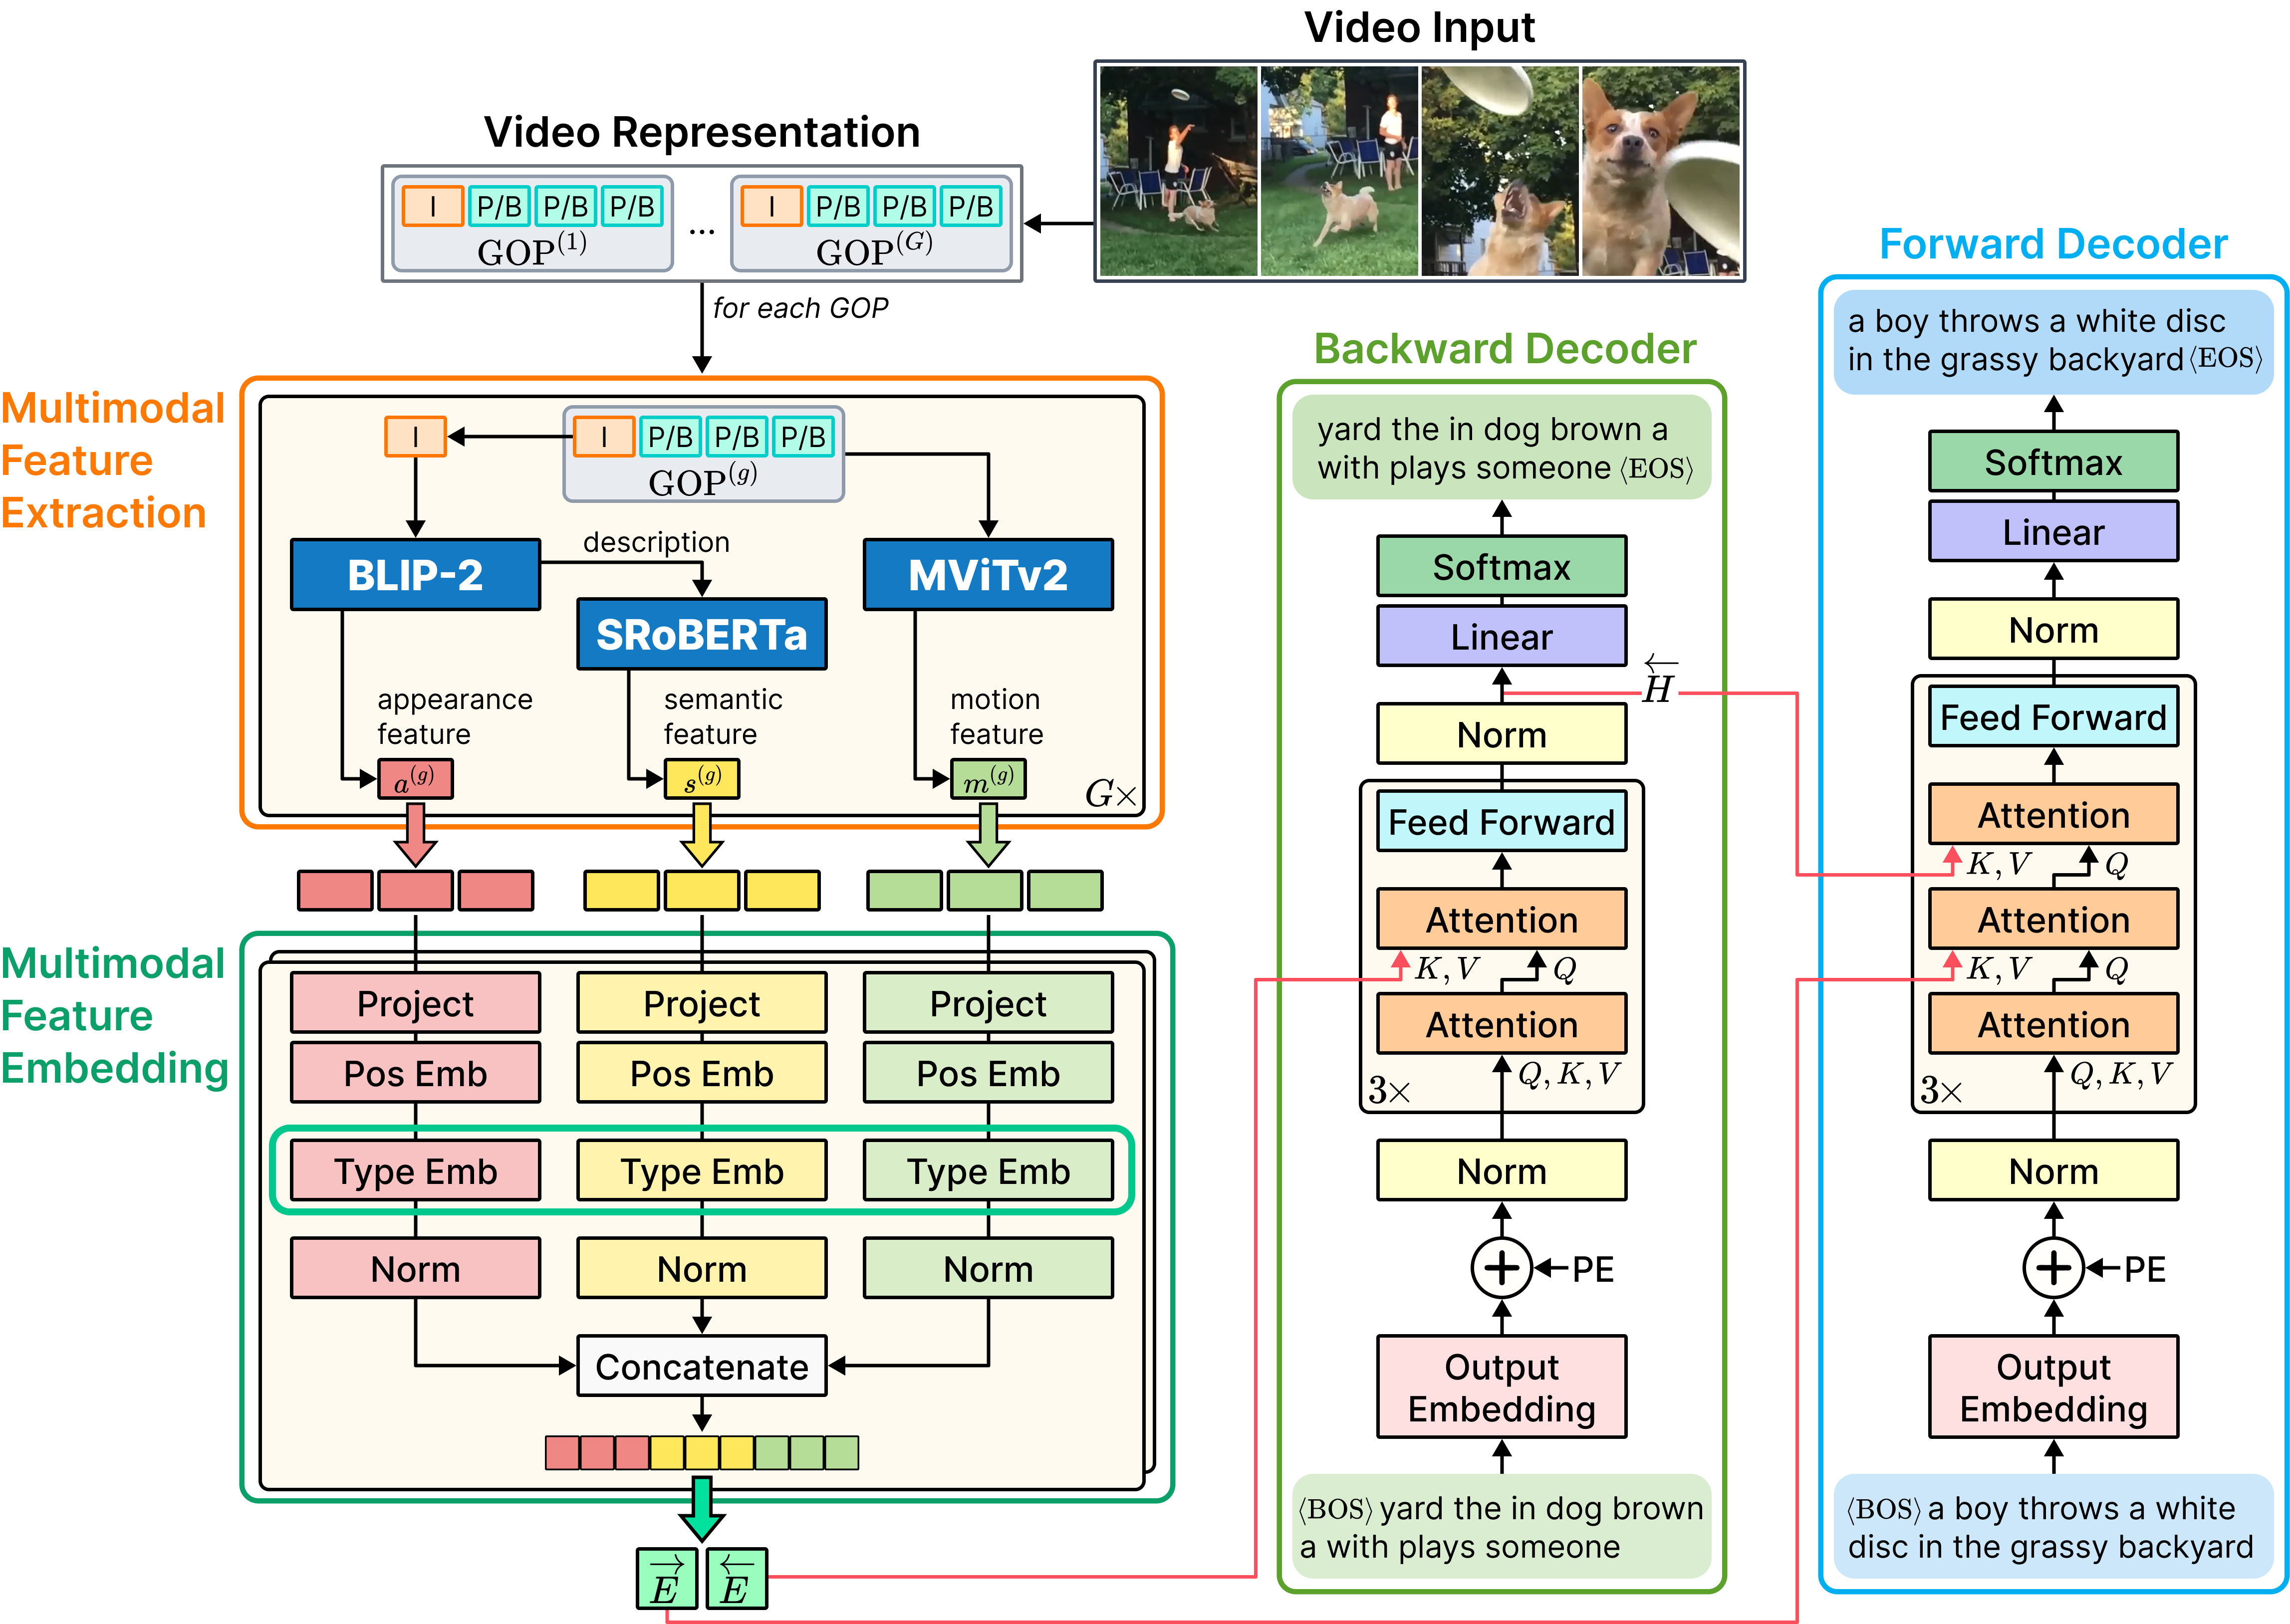
\includegraphics[width=0.99\columnwidth]{figures/fig04_overall_architecture.png}
\caption{Overview of the proposed BiDecT architecture. For each GOP, appearance features are extracted using BLIP-2, semantic features are obtained by encoding BLIP-2-generated descriptions with SRoBERTa, and motion features are extracted using MViTv2. These features are projected into a shared representation space and fused into a unified multimodal representation without any intermediate encoding stage. The Backward Decoder (BD) generates a reverse caption to construct a global backward contextual representation $\MyLVec[1]{H}$, while the Forward Decoder (FD) conditions on both the multimodal representation and $\MyLVec[1]{H}$ to generate the final caption.}
\label{fig:fig04_overall_architecture}
\end{figure}

\begin{figure*}[!t]
\centering
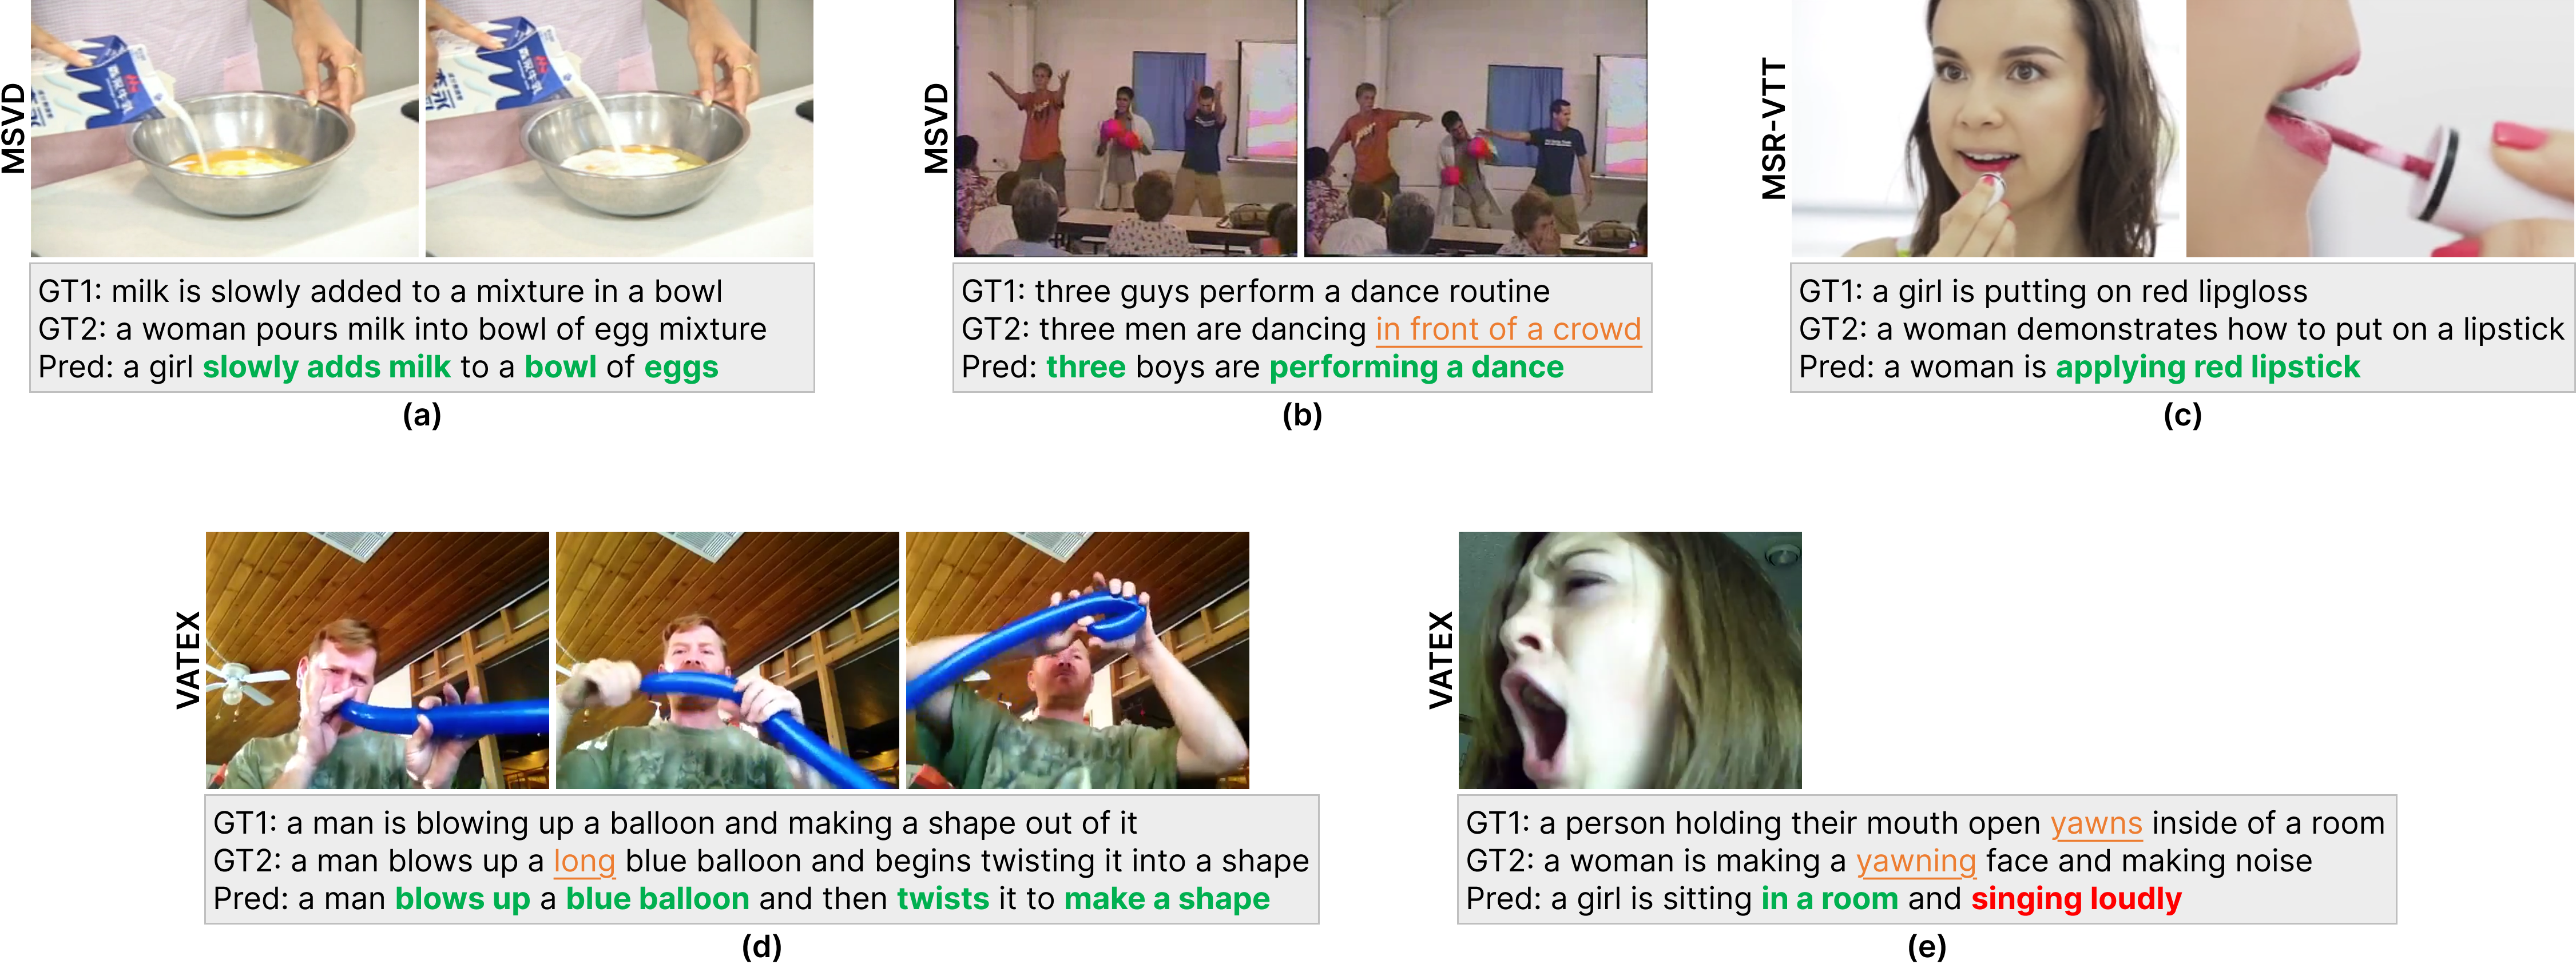
\includegraphics[width=0.99\textwidth, height=8.5in, keepaspectratio]{figures/fig10_case_study.png}
\caption{Qualitative examples of captions generated by BiDecT on MSVD, MSR-VTT, and VATEX. For each video, representative frames are shown alongside two ground-truth (GT) captions and the model prediction (Pred). {\textcolor[HTML]{00B050}{\textbf{Bold green text}}} denotes correctly predicted key terms; {\textcolor[HTML]{FF0000}{\textbf{bold red text}}} denotes hallucinated content; {\textcolor[HTML]{ED7D31}{\hluline{underlined orange text}}} in ground-truth captions marks important details not captured by the prediction. Examples (a)–(d) are success cases, example (e) is a failure case.}
\label{fig:fig10_case_study}
\end{figure*}

Text~\cite{banerjeeMETEORAutomaticMetric2005}

\bibliographystyle{IEEEtran}
\bibliography{references}


\end{document}
